\documentclass[10pt]{article}
\usepackage[letterpaper,margin=0.8in]{geometry}
\usepackage[T1]{fontenc}
\usepackage{lmodern}
\usepackage{microtype}
\usepackage{booktabs,tabularx,array}
\usepackage{url}
\usepackage[colorlinks=true,allcolors=blue]{hyperref}
\usepackage{pgfplots}
\pgfplotsset{compat=1.18}
\newcolumntype{Y}{>{\raggedright\arraybackslash}X}
\title{A Curated Local Collection of Market and Economic Time Series: A Dataset Card and Release Audit}
\author{Prakash Mallick\\\small Curation draft; owner confirmation required}
\date{9 October 2026}
\begin{document}
\maketitle

\begin{abstract}
This paper describes six local-only table products curated from agency publications and a documented crypto-market-data source. The products contain 99,216 physical table records: 2,465 timestamp-qualified economic events, 4,219 separately retained review events, 2,233 hourly Hyperliquid-derived bars, 4,084 Treasury-futures Traders in Financial Futures reports, 3,196 Australian government-yield observations, and 83,019 CFTC disaggregated futures-and-options reports. These counts combine tables with different observation semantics; they are neither unique aligned observations nor a count of fully timestamp-eligible records. The preparation manifest contains 54 files (106,875,828 bytes; about 106.9 MB). The CFTC disaggregated product is supplied as an 88 MB CSV and a 16,201,232-byte field-text Parquet companion; the two representations contain the same 83,019 records and are counted once. A broader filesystem inventory found 56,653 physical files occupying 241,884,028,581 bytes; the market category alone accounts for 236,633,734,490 bytes. The holdings include duplicate/package copies and model or analysis artifacts, so physical-file counts do not represent unique datasets. We describe schemas, temporal semantics, observed missingness, curation exclusions, source-rights qualifications, and known coverage limitations. No forecasting experiment or performance benchmark is reported.
\end{abstract}

\section{Motivation and scope}
Financial research datasets often combine observations with different clocks, units, publication lags, and reuse conditions. Documentation that makes these distinctions explicit is a practical prerequisite for responsible reuse, consistent with the dataset documentation framework proposed by Gebru et al.~\cite{gebru2021}. This paper is a dataset description and preparation audit: it records what the six retained tables contain and the conditions that limit their interpretation. It reports no model, prediction task, or benchmark result.

The collection joins event-level economic releases with financial-market and policy time series. It is a heterogeneous convenience collection, not a harmonized panel: rows do not share an observation cadence, instrument universe, unit, or common missing-data mechanism. The collection's event ledger also has two intentionally distinct tables. \texttt{economic\_events} records rows that passed a release-time evidence filter; \texttt{economic\_events\_review} preserves date-only items and rows whose release-time or revision status needs review. The latter must not be silently promoted to an intraday timestamped event sample.

\section{Preparation and availability}
Counts and schemas below are the values in the preparation's measured statistics snapshot. The 99,216 records are physical table rows across heterogeneous products, not unique, aligned, or uniformly timestamped observations: the 4,219 review-event rows include 4,129 records without a verified release instant, and the other tables represent hourly, weekly, daily, or date-only observations. A separate filesystem inventory records 56,653 physical files and 241,884,028,581 bytes across all categories. The market category accounts for 236,633,734,490 bytes and includes 27,131 Qlib-related physical copies; the broader holdings also contain packaged copies, archives, and model/analysis artifacts. Duplicate-group checks identified 1,072 verified groups. These physical counts and bytes describe discovered holdings; they are not a count of unique datasets.

The prepared copy is currently local and unpublished. It has no assigned DOI, public repository URL, or confirmed access endpoint. Availability is therefore limited to the local curation workspace until an owner authorizes a release location and each file's permission conditions are resolved. The preparation excludes source material held back because its provenance or redistribution rights are unresolved. In particular, a transformation log records that 577 FDIC rows were removed from the review-events input because redistribution rights for that source were unresolved; the FDIC failed-bank download is not included in the six products. We do not treat public visibility or a third-party dataset-card label as proof of redistribution rights.

\section{Dataset composition}
Table~\ref{tab:composition} summarizes row and column counts, time span, cadence, and units. Endpoint dates are recorded in the prepared statistics, but they do not imply that every date in the interval is represented. The CFTC disaggregated table is date-only and thus has no UTC offset in its dates. `UTC' in the other records refers to typed timestamps; it does not mean that source publications were originally issued in UTC.

\begin{table*}[t]
\centering\small
\caption{Measured composition of the six retained tables. Counts and date bounds are preparation-snapshot measurements.}
\label{tab:composition}
\begin{tabularx}{\textwidth}{@{}p{2.5cm} r r p{3.0cm} p{2.0cm} Y@{}}
\toprule
Table & Rows & Columns & Date bounds & Cadence & Contents and units \\
\midrule
Economic events & 2,465 & 37 & 2000-01-28--2026-09-16 & event-level & ABS and Federal Reserve release/document versions with explicit source release-time evidence; values retain source currency/unit. \\
Economic events review & 4,219 & 37 & publication dates 2000-01-05--2026-09-18 & event-level / review & AOFM, USDA, Federal Reserve, RBA and ABS records; includes 4,129 unknown-release-time rows and 90 revision-review rows. \\
Hyperliquid hourly & 2,233 & 9 & 2025-11-30 23:00--2025-12-31 23:00 UTC & hourly & BTC, ETH and SOL perpetual-trade OHLCVA; venue price/size units, amount is price times size, with no fiat conversion. \\
CFTC TFF & 4,084 & 20 & 2006-06-13--2025-12-30 & weekly reports & Four Treasury-futures instruments; positions and open interest in contracts. \\
RBA F2 & 3,196 & 7 & 2013-05-20--2025-12-31 & daily observations; weekly publication & Australian Government Security yields, in percent. \\
CFTC disaggregated & 83,019 & 191 & 2018-01-02--2024-12-31 & weekly reports & 543 instruments; source contract units vary and are represented by a source field. \\
\bottomrule
\end{tabularx}
\end{table*}

The two event tables share an event-oriented schema with identity and revision keys, event name/category, source provenance and evidence fields, UTC availability/release timestamps where supported, event date, quality status, and optional actual/forecast/prior values and surprise fields. The primary table's date range contains 2,465 typed timestamp rows. In the review table, only 90 rows have timestamp evidence; 4,129 rows have no verified release instant and remain review-only. The quality-status counts are 2,465 `eligible' rows in the primary table and, in the review table, 4,129 \texttt{unknown\_release\_time} plus 90 \texttt{source\_revision\_requires\_review}. The review set is not an alternative valid-time series.

The primary event table contains 1,581 ABS observations and 884 Federal Reserve observations. Its event categories are 1,581 scheduled-macro, 766 central-bank, and 118 credit/systemic records. As the category distribution shows, these labels describe curation categories rather than an exhaustive taxonomy of the underlying global economy. The review table is dominated by 3,307 AOFM policy/fiscal rows; it also contains 323 USDA, 312 Federal Reserve, 240 RBA and 37 ABS rows. These frequencies reflect what was assembled and the timestamp-quality filter, not source publication rates.

\subsection{Market and policy schemas}
The Hyperliquid-derived Parquet schema contains `item\_id', a timezone-aware timestamp, open/high/low/close, volume, amount and trade count. All nine measured columns have zero nulls in this 2,233-row snapshot. The upstream order-book dataset has a registered DataCite record and CC BY 4.0 rights metadata; the retained table is a derived hourly aggregation, not the upstream order-status or book-diff corpus~\cite{albers2026,dataciteapi}. Its short one-month, three-instrument coverage sharply limits inference about other coins, venues, or periods.

The CFTC TFF Parquet table has an instrument and market identity, observation and availability timestamps, open interest, and long/short/spread position fields for dealers, asset managers, leveraged money, other reportables and nonreportables. The 20 fields are complete in the measured snapshot. The 191-column disaggregated CSV preserves CFTC names and groups broad, old, and other report categories, positions, changes, percentages, and contract metadata; its 83,019 rows span 543 instruments. The statistics snapshot reports zero nulls for its two date/name identity fields only. It does not assert complete numeric fields. CFTC data are weekly reported positions, not transaction-level or daily trader holdings. Agency reuse guidance describes public-domain government information but excepts third-party contributions; attribution and artifact-level notice review remain necessary~\cite{cftctff,cftcterms}.

RBA F2 provides two timestamp fields and five yield series: 2-, 3-, 5-, and 10-year nominal yields and the 10-year indexed yield. Values are percentages. The measured table has 3,196 daily observations while publication follows a weekly schedule. Missing values are uneven by series: 98 each for the 2-, 3-, and 5-year columns; 20 for 10-year nominal; and 413 for 10-year indexed. The RBA's Financial Data terms expressly govern this table separately from general website licensing. They allow use under conditions, including attribution and no implication of endorsement, and reserve rights outside those permissions~\cite{rbaf2,rbaterms}.

\section{Time, nulls, and sampling}
The standardized event tables carry both a source-local timestamp string and typed UTC timestamp fields, alongside availability and ingestion timestamps. Those concepts are not interchangeable: an event's economic reference date, source publication instant, local source clock, and local ingestion time answer different questions. The event snapshot reports zero nulls in the typed event timestamp and availability timestamp columns for the primary table. By contrast, the review table has 4,129 nulls (out of 4,219) in each of `event\_timestamp\_local', `event\_timestamp\_utc', and `available\_timestamp'. Date-only CFTC rows are intentionally left as dates rather than assigned invented times.

Missingness is substantively informative. For example, the primary event table has 2,395 missing values in each of `actual\_value' and `unit'; forecast, prior, revised-prior, surprise and normalized-surprise are missing for all 2,465 rows. This reflects a release/document-version ledger where event identity and timing evidence can be present without a numeric macro release value. In the review table, 896 rows lack actual values, whereas forecast and prior values are absent for all 4,219. The measures should not be interpreted as a balanced panel of consensus forecasts and realizations.

\begin{figure}[t]
\centering
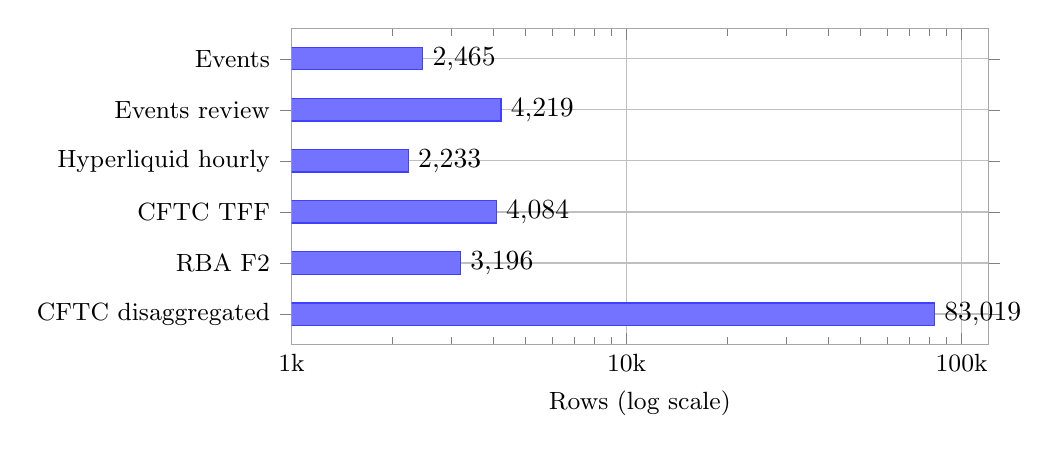
\begin{tikzpicture}
\begin{axis}[
  xbar, width=0.86\linewidth, height=5.6cm, point meta=rawx,
  xlabel={Rows (log scale)}, xmode=log,
  xmin=1000, xmax=120000,
  symbolic y coords={Events,Events review,Hyperliquid hourly,CFTC TFF,RBA F2,CFTC disaggregated},
  ytick=data, y dir=reverse, nodes near coords, nodes near coords align={horizontal},
  tick label style={font=\small}, label style={font=\small},
  bar width=8pt, enlarge y limits=0.12,
  xtick={1000,10000,100000}, xticklabels={1k,10k,100k},
  grid=major, axis line style={gray!70}
]
\addplot[fill=blue!55,draw=blue!75] coordinates {
 (2465,Events) (4219,Events review) (2233,Hyperliquid hourly)
 (4084,CFTC TFF) (3196,RBA F2) (83019,CFTC disaggregated)
};
\end{axis}
\end{tikzpicture}
\caption{Table row counts on a logarithmic axis. The graphic emphasizes scale differences and does not indicate temporal continuity or statistical comparability.}
\label{fig:rows}
\end{figure}

\section{Provenance and rights boundaries}
The six tables are sourced from official Australian and US statistical or policy sources, CFTC reports, and a separately documented Hyperliquid-derived hourly file. ABS website-produced material generally carries CC BY 4.0 subject to exclusions; the Federal Reserve Board states that its website information is public domain unless otherwise indicated; CFTC government information is public domain with requested acknowledgment, subject to third-party-material exceptions. The RBA F2 Financial Data terms are distinct from its general copyright terms. AOFM and USDA materials are retained only with the conditions and artifact-level qualifications noted in the audit~\cite{absrights,fedrights,aofmrights,usdarecord,nalrights}.

The release audit excluded material with unresolved or incompatible reuse conditions. For example, the local Kaggle record labels a Coinbase-derived dataset CC0, but Coinbase's own Market Data Terms restrict redistribution and derived works. Those two claims do not settle the source-rights chain, so the Coinbase/Kaggle corpus is not part of this collection~\cite{coinbasekaggle,coinbaseterms}. The same principle applies to research and exchange data: FI-2010 has a published benchmark paper and an official Fairdata record, but it is not included here; Binance Vision terms specify a noncommercial, share-alike license rather than an unrestricted release; and the Qlib-heavy holdings counted in filesystem inventory are not included as independent datasets~\cite{ntakaris2018,fi2010fairdata,binanceterms}. This paper documents an audit decision, not a legal opinion or a claim that every allowed use is settled.

\section{Appropriate uses and limitations}
The tables can support descriptive work that respects the native cadence and source units: analysis of event-source timing evidence, weekly CFTC positioning, short historical OHLC summaries for three perpetual instruments, or descriptive examination of RBA yield-series coverage. Research design should preserve availability times when constructing point-in-time information sets and should treat the event review table as an uncertainty stratum, not as confirmed intraday event timestamps.

The collection is not representative of all markets, releases, assets, participant populations, or time periods. The crypto sample covers approximately one month and only BTC/ETH/SOL; the RBA series cover a selected maturity set; CFTC reports are thresholded, weekly aggregate disclosures; economic releases have source and timestamp selection biases; and source revisions or publication calendars can change. Null counts indicate observed completeness in one measured copy, not correctness or absence of measurement error. No data quality adjudication beyond the documented schema, counts, provenance, and quality flags is claimed.

The upstream order-book source contains wallet identifiers in its raw order/trade streams. Those wallet identifiers are not included in the retained hourly OHLC table, which aggregates instrument-hour bars. This is a schema-level distinction, not a broad anonymization guarantee for other files. Avoid attempts to identify individuals, link pseudonymous activity to real identities, or infer sensitive personal attributes from public wallet activity. The CFTC and macro tables are published aggregates but still require careful interpretation and attribution.

\section{Ethics and maintenance}
The preparation snapshot is frozen for this draft and dated 9 October 2026. It has not yet been published. Before release, the owner should verify authorship, affiliation, access location, current upstream terms and artifact notices, and whether the intended use requires narrower redistribution or data-derived outputs. Re-running the curation should regenerate the statistics, schema files, inventory, and transformation record from an identified snapshot; changing an upstream source or source-rights outcome should result in a versioned release and refreshed documentation. The paper intentionally leaves repository and DOI fields absent rather than assigning identifiers to an unpublished local copy.

\section*{Data availability}
The described preparation is local and unpublished as of the paper date. No public download URL or DOI is assigned. The preparation manifest contains 54 files (106,875,828 bytes). It includes both the CFTC disaggregated CSV (about 88 MB) and a 16,201,232-byte field-text Parquet representation. They encode the same 83,019 records, counted once among the six table products. Availability beyond the local workspace awaits owner confirmation and completion of applicable source-level and artifact-level checks.

\section*{Author contributions and competing interests}
The draft credits Prakash Mallick as curator, subject to owner confirmation before submission. The curation workflow assembled, filtered, measured and documented the tables. No competing-interest statement has been confirmed; this field requires owner review.

\begin{thebibliography}{99}
\bibitem{gebru2021} T. Gebru, J. Morgenstern, B. Vecchione, J. W. Vaughan, H. Wallach, H. Daum\'{e} III, and K. Crawford, ``Datasheets for Datasets,'' \emph{Communications of the ACM}, 64(12), 86--92, 2021. \url{https://doi.org/10.1145/3458723}. Preprint: \url{https://arxiv.org/abs/1803.09010}.
\bibitem{albers2026} J. Albers, M. Cucuringu, S. Howison, and A. Y. Shestopaloff, \emph{An Open Book: Level 4 Order Book Data from the Hyperliquid Exchange}, Zenodo, version 1.0, 2026. \url{https://doi.org/10.5281/zenodo.18184441}. DataCite record lists four creators and CC BY 4.0 rights metadata.
\bibitem{dataciteapi} DataCite, ``REST API: Retrieve a single DOI,'' \url{https://support.datacite.org/docs/api-get-doi}; live record queried at \url{https://api.datacite.org/dois/10.5281/zenodo.18184441}.
\bibitem{cftctff} U.S. Commodity Futures Trading Commission, ``Traders in Financial Futures,'' official public data portal, \url{https://publicreporting.cftc.gov/stories/s/TFF-Futures/98ig-3k9y/}.
\bibitem{cftcterms} U.S. Commodity Futures Trading Commission, ``Terms of Use Agreement,'' section ``Reproduction of CFTC Content,'' \url{https://accountcreation.cftc.gov/TermsOfUseAgreement.aspx}.
\bibitem{rbaf2} Reserve Bank of Australia, ``Statistical Table F2: Capital Market Yields--Government Bonds--Daily,'' \url{https://www.rba.gov.au/statistics/tables/}.
\bibitem{rbaterms} Reserve Bank of Australia, ``Copyright and Disclaimer Notice,'' section 5, Financial Data terms and conditions, \url{https://www.rba.gov.au/copyright/index.html}.
\bibitem{absrights} Australian Bureau of Statistics, ``Website privacy, copyright and disclaimer,'' \url{https://www.abs.gov.au/website-privacy-copyright-and-disclaimer}.
\bibitem{fedrights} Board of Governors of the Federal Reserve System, ``Disclaimer,'' \url{https://www.federalreserve.gov/disclaimer.htm}.
\bibitem{aofmrights} Australian Office of Financial Management, ``Copyright,'' \url{https://www.aofm.gov.au/copyright}.
\bibitem{usdarecord} USDA World Agricultural Outlook Board, ``World Agricultural Supply and Demand Estimates,'' Economic Research Service Market Information System, \url{https://esmis.nal.usda.gov/publication/world-agricultural-supply-and-demand-estimates}.
\bibitem{nalrights} U.S. National Agricultural Library, ``Web policies and important links,'' \url{https://www.nal.usda.gov/web-policies-and-important-links}.
\bibitem{coinbasekaggle} Kaggle, ``High Frequency Crypto Limit Order Book Data,'' dataset metadata record, \url{https://www.kaggle.com/datasets/martinsn/high-frequency-crypto-limit-order-book-data}. The Kaggle license label alone does not resolve underlying provider rights.
\bibitem{coinbaseterms} Coinbase, ``Market Data Terms of Use,'' \url{https://www.coinbase.com/legal/market_data}.
\bibitem{ntakaris2018} A. Ntakaris, M. Magris, J. Kanniainen, M. Gabbouj, and A. Iosifidis, ``Benchmark dataset for mid-price forecasting of limit order book data with machine learning methods,'' \emph{Journal of Forecasting}, 37(8), 852--866, 2018. \url{https://doi.org/10.1002/for.2543}; preprint \url{https://arxiv.org/abs/1705.03233}.
\bibitem{fi2010fairdata} Finnish Fairdata Etsin, ``Benchmark Dataset for Mid-Price Forecasting of Limit Order Book Data,'' official dataset record, \url{https://etsin.fairdata.fi/dataset/73eb48d7-4dbc-4a10-a52a-da745b47a649}.
\bibitem{binanceterms} Binance, ``Vision Dataset Terms and Conditions,'' official source repository, \url{https://github.com/binance/binance-public-data/blob/master/TERMS_AND_CONDITIONS.md}; market data archives at \url{https://data.binance.vision/}.
\end{thebibliography}
\end{document}
